\documentclass[10pt,aspectratio=169]{beamer}

\usetheme[progressbar=foot]{metropolis}
\AtBeginSection{}

\usepackage{appendixnumberbeamer}
\usepackage{booktabs}
\usepackage[scale=2]{ccicons}
\usepackage{tabularx}
\usepackage{tikz}
\usetikzlibrary{arrows.meta,positioning,shapes.geometric,fit,calc}
\usepackage{xspace}
\newcommand{\themename}{\textbf{\textsc{metropolis}}\xspace}
\usepackage{comment}
\usepackage{caption}
\usepackage[
  backend=biber,
  style=authoryear
]{biblatex}

\setbeamertemplate{bibliography item}{}
\addbibresource{bibliography.bib}

\usepackage{graphicx}
\usepackage{siunitx}



%................................................................................
% COLORS

\definecolor{ukudlaBlue}{RGB}{41, 60, 135}
\definecolor{ukudlaLightBlue}{RGB}{212, 216, 231}
\definecolor{ukudlaRed}{RGB}{164, 28, 34}
\definecolor{ukudlaLightRed}{RGB}{236, 209, 210}
\definecolor{ukudlaGreen}{RGB}{59, 139, 71}
\definecolor{ukudlaLightGreen}{RGB}{215, 231, 218}
\definecolor{ukudlaYellow}{RGB}{239, 198, 44}
\definecolor{ukudlaLightYellow}{RGB}{251, 243, 212}
\definecolor{white}{RGB}{255, 255, 255}
\definecolor{black}{RGB}{0, 0, 0}

\setbeamercolor{palette primary}{fg=white, bg=ukudlaGreen}
\setbeamercolor{progress bar}{fg=ukudlaRed, bg=ukudlaYellow}
\setbeamercolor{title separator}{fg=ukudlaRed, bg=ukudlaYellow}
\setbeamercolor{progress bar in head/foot}{fg=ukudlaRed, bg=ukudlaYellow}
\setbeamercolor{progress bar in section page}{fg=ukudlaRed, bg=ukudlaYellow}
\setbeamercolor{background canvas}{bg=white}
\setbeamercolor{block body}{bg=ukudlaLightGreen,fg=black}



%................................................................................
% PRESENTATION INFORMATION

\title{UKUDLA Data Science Certificate}
\subtitle{Data Preparation}
\author{Markus Mößler}
\institute{University of Hohenheim}



%................................................................................
% CUSTOM FOOTER

\makeatletter
\setbeamertemplate{progress bar in head/foot}{%
  \tikzset{metropolis@progressbar@foreground/.style={fill=ukudlaGreen}}%
  \tikzset{metropolis@progressbar@background/.style={fill=ukudlaLightGreen}}%

  \begin{tikzpicture}[overlay, x=\paperwidth, y=1cm]
    \fill[metropolis@progressbar@background]
      (0,0) rectangle (1,0.10);
    \fill[metropolis@progressbar@foreground]
      (0,0) rectangle
      ({\insertframenumber/\inserttotalframenumber},0.10);
    \node[anchor=south west, yshift=0.25cm, xshift=0.2cm]
      at (0,0)
      {\includegraphics[height=0.75cm]{./logos/UKUDLA_logo_03_white_bg.pdf}};
    % current section
    \ifnum\value{section}>0
      \node[
        anchor=south east,
        yshift=0.22cm,
        xshift=-0.60cm,
        fill=ukudlaLightGreen,
        rounded corners=2pt,
        inner xsep=6pt,
        inner ysep=3pt,
        font=\scriptsize\bfseries,
        text=ukudlaRed
      ] at (1,0) {
        \insertsectionhead
      };
    \fi

  \end{tikzpicture}%
}
\makeatother



%................................................................................
% CUSTOM TITLE PAGE

\makeatletter
\setbeamertemplate{title page}{
  \begin{beamercolorbox}[sep=8pt, center, wd=\paperwidth, ht=0.5\paperheight]{title page top}
    \begin{minipage}[c]{1.00\textwidth}
      \raggedleft
      \includegraphics[height=1.00cm]{./logos/ukudla_universities.pdf}
      \vspace*{0.2cm}
    \end{minipage}
    \begin{beamercolorbox}[wd=0.9\paperwidth, sep=12pt, left]{top box}
      {\usebeamerfont{title}\usebeamercolor[fg]{title}\inserttitle\par}
      \vskip0.1cm
      {\usebeamerfont{subtitle}\usebeamercolor[fg]{subtitle}\insertsubtitle\par}
    \end{beamercolorbox}
  \end{beamercolorbox}
  \begin{beamercolorbox}[sep=8pt, center, wd=\paperwidth, ht=0.5\paperheight]{title page bottom}
    \begin{beamercolorbox}[wd=0.9\paperwidth, sep=12pt, left]{bottom box}
      \hbox{%
        \hspace*{1em}
        \begin{minipage}[c]{0.40\textwidth}
          \vskip1.0cm
          {\usebeamerfont{author}\usebeamercolor[fg]{author}\insertauthor\par}
          \vskip0.1cm
          {\usebeamerfont{institute}\usebeamercolor[fg]{institute}\insertinstitute\par}
        \end{minipage}%
        \hspace*{1.5cm}
        \begin{minipage}[c]{1.00\textwidth}
          \includegraphics[height=2.0cm]{./logos/UKUDLA_logo_05.pdf}
        \end{minipage}%
      }
    \end{beamercolorbox}
    \begin{minipage}[r]{1.00\textwidth}
      \centering
      \includegraphics[width=1.00\textwidth]{./logos/ukudla_sponsors.pdf}
    \end{minipage}
  \end{beamercolorbox}
}
\makeatother

\setbeamercolor{title page top}{bg=white}
\setbeamercolor{top box}{bg=ukudlaGreen}
\setbeamercolor{title page bottom}{bg=white}
\setbeamercolor{bottom box}{bg=ukudlaLightGreen}
\setbeamercolor{title}{fg=white}
\setbeamercolor{subtitle}{fg=white}
\setbeamercolor{author}{fg=black}
\setbeamercolor{institute}{fg=black}
\setbeamercolor{date}{fg=black}



%................................................................................
% DOCUMENT

\begin{document}

\maketitle

%--------------------------------------------------
{
\setbeamertemplate{frame numbering}[none]

\begin{frame}[noframenumbering]{Table of contents}

  \small
  \setbeamertemplate{section in toc}[sections numbered]
  \tableofcontents[hideallsubsections]

\end{frame}
}
%--------------------------------------------------



\section{Motivation}


%--------------------------------------------------
% CONTENT SLIDE 1/10
\begin{frame}{Integrated data are not automatically analysis-ready}

\small

\begin{columns}[T]

\column{0.47\textwidth}

\textbf{The sources are managed and joined}

\begin{itemize}
  \item inputs are identified and documented;
  \item keys and coverage are validated;
  \item identifiers, space and time are aligned; and
  \item the join is audited.
\end{itemize}

\column{0.48\textwidth}

\textbf{The analysis still needs decisions}

\begin{itemize}
  \item which observations are retained?
  \item which shape should the table have?
  \item which units and types are required?
  \item which variables should be derived?
\end{itemize}

\end{columns}

\vspace{0.35cm}

\begin{beamercolorbox}[rounded=true,sep=8pt]{block body}
Data preparation turns managed evidence into a documented representation suited to a defined analysis.
\end{beamercolorbox}

\end{frame}
%--------------------------------------------------


%--------------------------------------------------
% CONTENT SLIDE 2/10
\begin{frame}{Preparation choices affect the result}

\small
\centering

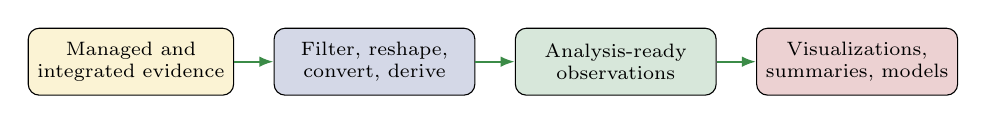
\begin{tikzpicture}[
  artifact/.style={
    draw,
    rounded corners,
    minimum width=2.55cm,
    minimum height=0.85cm,
    align=center,
    font=\scriptsize
  },
  arrow/.style={-{Latex[length=1.8mm]},thick,ukudlaGreen}
]
  \node[artifact,fill=ukudlaLightYellow] (evidence) {Managed and\\integrated evidence};
  \node[artifact,fill=ukudlaLightBlue,right=0.50cm of evidence] (decisions) {Filter, reshape,\\convert, derive};
  \node[artifact,fill=ukudlaLightGreen,right=0.50cm of decisions] (analysis) {Analysis-ready\\observations};
  \node[artifact,fill=ukudlaLightRed,right=0.50cm of analysis] (results) {Visualizations,\\summaries, models};
  \draw[arrow] (evidence) -- (decisions);
  \draw[arrow] (decisions) -- (analysis);
  \draw[arrow] (analysis) -- (results);
\end{tikzpicture}

\vspace{0.55cm}

\raggedright

\begin{itemize}
  \item Dropping a record changes the population represented.
  \item Aggregation hides variation and requires a summary rule.
  \item Unit conversion changes values but should preserve meaning.
  \item Derived variables encode assumptions that later results inherit.
\end{itemize}

\vspace{0.15cm}

\begin{beamercolorbox}[rounded=true,sep=8pt]{block body}
This session moves from \textbf{motivation}, through the essential
\textbf{concepts}, to a reproducible \textbf{application} for an analytical dataset.
\end{beamercolorbox}

\end{frame}
%--------------------------------------------------



\section{Concepts}


%--------------------------------------------------
% CONTENT SLIDE 3/10
\begin{frame}{Related activities answer different questions}

\scriptsize

\begin{tabularx}{\textwidth}{lXX}
\toprule
\textbf{Activity} & \textbf{Central question} & \textbf{Typical evidence} \\
\midrule
Validation & Do data meet documented expectations? & Checks and findings \\
Cleaning & Is a value demonstrably erroneous, and how is it corrected? & Justified correction record \\
Integration & How are compatible observations connected across sources? & Join contract and audit \\
Preparation & How are data represented for the intended analysis? & Reproducible transformations \\
\bottomrule
\end{tabularx}

\vspace{0.45cm}

\small

\begin{beamercolorbox}[rounded=true,sep=8pt]{block body}
A surprising value is not automatically an error. Preserve the evidence, investigate its meaning, and separate correction from transformation.
\end{beamercolorbox}

\end{frame}
%--------------------------------------------------


%--------------------------------------------------
% CONTENT SLIDE 4/10
\begin{frame}{Begin with the target observation}

\small

\begin{columns}[T]

\column{0.43\textwidth}

\textbf{Analysis contract}

Before transforming, state:

\begin{itemize}
  \item intended population;
  \item observation grain;
  \item candidate key;
  \item outcome and other variables;
  \item units and time periods; and
  \item missing-value policy.
\end{itemize}

\column{0.53\textwidth}

\begin{beamercolorbox}[rounded=true,sep=8pt]{block body}
\textbf{Example analysis target}

\vspace{0.10cm}

One row represents one region and year, containing an outcome and explanatory measures aligned to that period.

\vspace{0.15cm}

\textbf{Candidate key}

\texttt{region\_id + year}
\end{beamercolorbox}

\end{columns}

\vspace{0.35cm}

\centering
\textcolor{ukudlaRed}{The target grain determines which transformations are valid.}

\end{frame}
%--------------------------------------------------


%--------------------------------------------------
% CONTENT SLIDE 5/10
\begin{frame}{Reshape structure without hiding meaning}

\small

\begin{columns}[T]

\column{0.46\textwidth}

\textbf{Long source representation}

\begin{tabularx}{\textwidth}{lXX}
\toprule
Unit & Measure & Value \\
\midrule
Plot 12 & Biomass & 2.34 \\
Plot 12 & Soil moisture & 18.6 \\
Plot 12 & Nitrogen & 40 \\
\bottomrule
\end{tabularx}

\column{0.50\textwidth}

\textbf{Wide analytical representation}

\begin{tabularx}{\textwidth}{lXX}
\toprule
Unit & Biomass & Soil moisture \\
\midrule
Plot 12 & 2.34 & 18.6 \\
\bottomrule
\end{tabularx}

\vspace{0.20cm}

One target unit becomes one row with a separate variable for each retained measure.

\end{columns}

\vspace{0.35cm}

\begin{beamercolorbox}[rounded=true,sep=8pt]{block body}
Reshaping is valid only after the source key is known and every output cell is expected to receive at most one value.
\end{beamercolorbox}

\end{frame}
%--------------------------------------------------


%--------------------------------------------------
% CONTENT SLIDE 6/10
\begin{frame}{Make every transformation explicit}

\scriptsize

\begin{tabularx}{\textwidth}{lXX}
\toprule
\textbf{Operation} & \textbf{Question} & \textbf{Evidence to preserve} \\
\midrule
Select/filter & Which population and variables remain? & Inclusion rule and row counts \\
Parse/recode & How are types, dates, labels or codes interpreted? & Mapping and failed parses \\
Convert & Are definitions and dimensions compatible? & Formula, source and target units \\
Reshape & What becomes an observation or variable? & Input and output grain and keys \\
Handle missingness & Is absence unknown, structural or introduced? & Missingness before and after \\
Derive & What assumption defines the new variable? & Formula, inputs and valid domain \\
\bottomrule
\end{tabularx}

\vspace{0.40cm}

\small

\begin{beamercolorbox}[rounded=true,sep=8pt]{block body}
Do not silently delete duplicates, replace missing values, cap outliers, or coerce failed values merely to make code complete.
\end{beamercolorbox}

\end{frame}
%--------------------------------------------------


\section{Application}


%--------------------------------------------------
% CONTENT SLIDE 7/10
\begin{frame}{Preparation can occur around integration}

\small
\centering

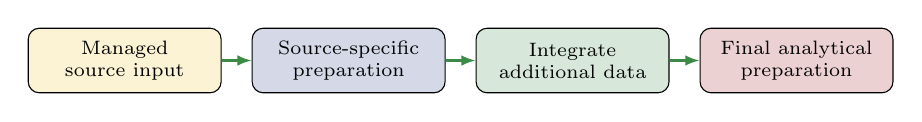
\begin{tikzpicture}[
  artifact/.style={
    draw,
    rounded corners,
    minimum width=2.45cm,
    minimum height=0.82cm,
    align=center,
    font=\scriptsize
  },
  arrow/.style={-{Latex[length=1.8mm]},thick,ukudlaGreen}
]
  \node[artifact,fill=ukudlaLightYellow] (fao) {Managed\\source input};
  \node[artifact,fill=ukudlaLightBlue,right=0.38cm of fao] (panel) {Source-specific\\preparation};
  \node[artifact,fill=ukudlaLightGreen,right=0.38cm of panel] (integrate) {Integrate\\additional data};
  \node[artifact,fill=ukudlaLightRed,right=0.38cm of integrate] (final) {Final analytical\\preparation};
  \draw[arrow] (fao) -- (panel);
  \draw[arrow] (panel) -- (integrate);
  \draw[arrow] (integrate) -- (final);
\end{tikzpicture}

\vspace{0.55cm}

\raggedright

\begin{itemize}
  \item Source-specific preparation makes source grains compatible.
  \item Integration connects compatible observations across sources.
  \item Final preparation selects or derives variables for a stated analysis.
  \item Each stage writes a new artifact; no stage edits a managed input.
\end{itemize}

\vspace{0.20cm}

\centering
\textcolor{ukudlaRed}{Workflow order is determined by dependencies, not by topic boundaries.}

\end{frame}
%--------------------------------------------------


%--------------------------------------------------
% CONTENT SLIDE 8/10
\begin{frame}{Prepare an analysis-specific dataset}

\small

\begin{columns}[T]

\column{0.47\textwidth}

\textbf{Validate before reshaping}

\begin{itemize}
  \item expected variable--unit pairs;
  \item unique unit--occasion--measure keys;
  \item known unit, treatment and period coverage; and
  \item numeric values and missingness.
\end{itemize}

\column{0.47\textwidth}

\textbf{Transform deliberately}

\begin{itemize}
  \item retain observations relevant to the question;
  \item reshape measures into analytical variables;
  \item harmonize units under documented formulas;
  \item derive transformations only on valid domains; and
  \item arrange one row per target observation.
\end{itemize}

\end{columns}

\vspace{0.35cm}

\begin{beamercolorbox}[rounded=true,sep=8pt]{block body}
The conversion formula, log domain, output grain, row count and candidate key are part of the preparation contract.
\end{beamercolorbox}

\end{frame}
%--------------------------------------------------


%--------------------------------------------------
% CONTENT SLIDE 9/10
\begin{frame}{Audit preparation and preserve lineage}

\small

\begin{columns}[T]

\column{0.47\textwidth}

\textbf{Preparation audit}

\begin{itemize}
  \item input and output rows;
  \item unique input and output keys;
  \item failed parses or mappings;
  \item missingness before and after;
  \item valid units and ranges; and
  \item unchanged managed inputs.
\end{itemize}

\column{0.47\textwidth}

\textbf{Lineage record}

\begin{itemize}
  \item input and output artifacts;
  \item script and relevant parameters;
  \item filters and reshaping rules;
  \item conversion and derivation formulas;
  \item information lost; and
  \item dictionary updates.
\end{itemize}

\end{columns}

\vspace{0.35cm}

\begin{beamercolorbox}[rounded=true,sep=8pt]{block body}
Transformations learned from observed distributions---such as imputation or scaling---must later be estimated from training data only to prevent leakage.
\end{beamercolorbox}

\end{frame}
%--------------------------------------------------


%--------------------------------------------------
\section{Key Message}
% CONTENT SLIDE 10/10

\begin{frame}{Key message: analysis-ready is purpose-specific}

\small

\centering

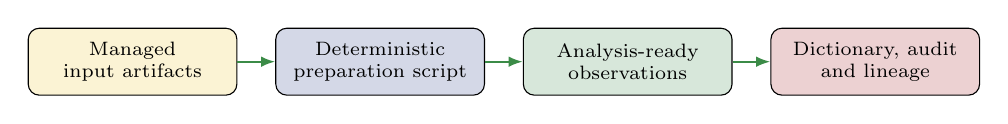
\begin{tikzpicture}[
  artifact/.style={
    draw,
    rounded corners,
    minimum width=2.65cm,
    minimum height=0.85cm,
    align=center,
    font=\scriptsize
  },
  arrow/.style={-{Latex[length=1.8mm]},thick,ukudlaGreen}
]
  \node[artifact,fill=ukudlaLightYellow] (inputs) {Managed\\input artifacts};
  \node[artifact,fill=ukudlaLightBlue,right=0.48cm of inputs] (script) {Deterministic\\preparation script};
  \node[artifact,fill=ukudlaLightGreen,right=0.48cm of script] (data) {Analysis-ready\\observations};
  \node[artifact,fill=ukudlaLightRed,right=0.48cm of data] (evidence) {Dictionary, audit\\and lineage};
  \draw[arrow] (inputs) -- (script);
  \draw[arrow] (script) -- (data);
  \draw[arrow] (data) -- (evidence);
\end{tikzpicture}

\vspace{0.45cm}

\raggedright

\begin{enumerate}
  \item State the target population, grain, key, variables and units.
  \item Validate each assumption before applying its transformation.
  \item Write derived artifacts instead of editing managed inputs.
  \item Check row counts, keys, missingness, units and valid domains.
  \item Document how every output variable was created.
\end{enumerate}

\vspace{0.15cm}

\centering
\textcolor{ukudlaRed}{Analysis-ready means ready for a stated purpose---not universally clean or final.}

\end{frame}
%--------------------------------------------------


%--------------------------------------------------
\begin{frame}[plain,noframenumbering]{Supported by}

  South African government and the National Research Foundation

  \begin{flushleft}
    \includegraphics[trim=0cm 0cm 0cm 0cm, clip, width=0.50\textwidth]{./logos/ukudla_south_african_sponsors.pdf}
  \end{flushleft}

  German government and the German Academic Exchange Service

  \begin{flushleft}
    \includegraphics[trim=0cm 0cm 0cm 0cm, clip, width=1.00\textwidth]{./logos/ukudla_german_sponsors.pdf}
  \end{flushleft}

\end{frame}
%--------------------------------------------------

\end{document}
